\section{Benutzeroberfläche}
 In diesem Kapitel wird die Benutzeroberfläche der \gls{gbta} sowie ein 
 entsprechender Entwurfsvorschlag vorgestellt.

\begin{figure}[ht]
	\begin{center}
	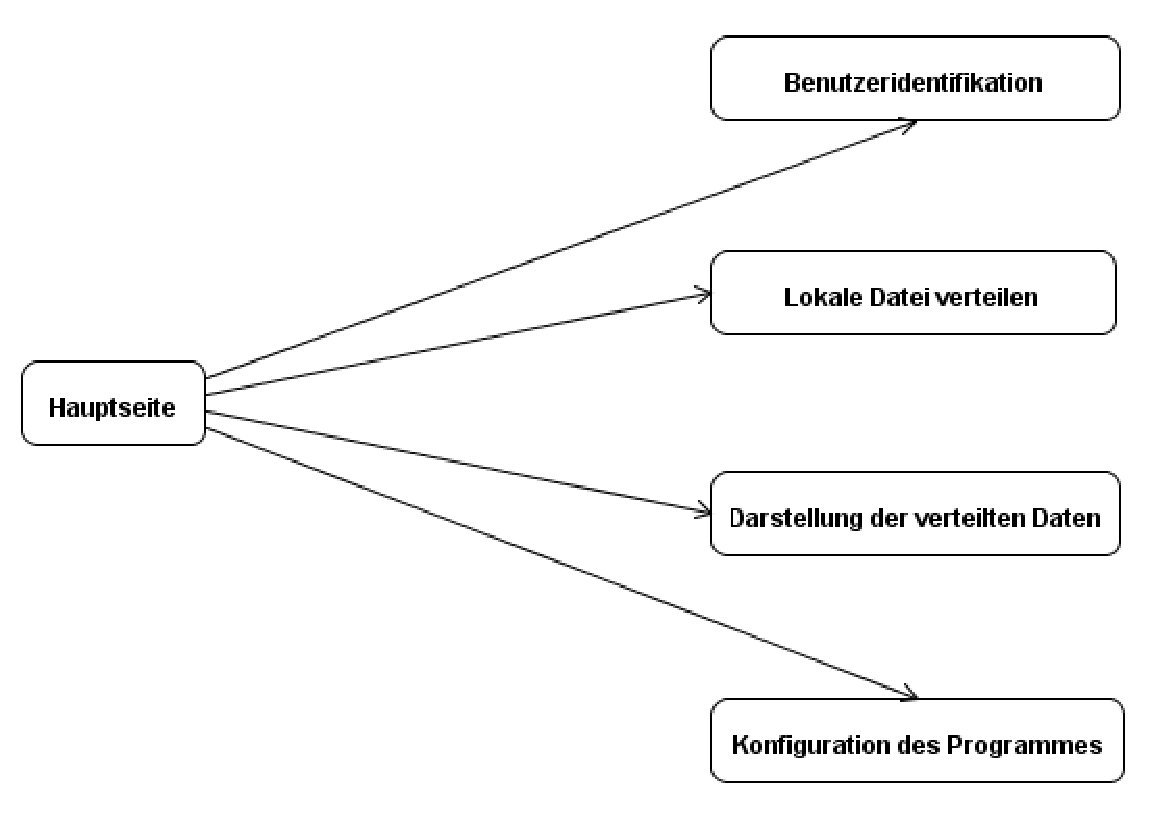
\includegraphics[scale=0.8]{GUIZentral}	
	\end{center}
	\caption{Die Benutzeroberfläche (schematisch).}
\end{figure}

  \subsection{Dialogstruktur}
  Für die Benutzerführung ist die nachfolgende Dialogstruktur vorgesehen, die sich aus 
  den nachfolgenden Komponenten zusammensetzt:
  \begin{enumerate}[1.)]
   \item Einem Dialog zum Anmelden an das System. Eine Abmeldung ist nicht vorgesehen. Eingabe ist die
Benutzerkennung sowie ein Kennwort.

   \item Eine Dialogbox wird verwendet für die Konfiguration von BaseTorrent, d.h. der Eingabe eines Verzeichnisses,
der beim Ablegen von verteilten Dateien und Ordnern verwendet wird. Zudem wird eine maximale Speichergröße
  als auch ein zusätzliches Verzeichnis hinterlegt. Beides wird herangezogen um anderen Benutzern auf dem
  vorliegenden Rechner Speicherkapazität zum Verteilen von Dateien im Netzwerk bereitzustellen.

   \item Die Darstellung von bereits veröffentlichten Dateien und Ordnern sowie, sofern der Benutzer sich gemäß 1.)
  angemeldet hat, auch der benutzerbezogenen Daten.  Diese können in zwei separaten, wenn auch weitestgehend
identisch aufgebauten Komponenten dargestellt werden.

   \item Eine Dialogbox zeigt den Fortschritt des Speicherns von verteilten Daten (der sogenannte \emph{Download}) an.
   \item Eine weitere Dialogbox zeigt ein Eingabefeld an, um nach Dateien mit einem bestimmten Schlüsselwort zu suchen.
  \end{enumerate}

  \subsection{Bildschirmlayout}
  Um eine intuitive Benutzerführung zu gewährleisten wird ein Layout entsprechend 
  der Programmierrichtlinien für die Gestaltung der Benutzeroberflächen von  
  Desktop-Applikationen angestrebt\footnote{Etwa \emph{Microsoft Inductive User Interface Guidelines, http://msdn.microsoft.com/en-us/library/ms997506.aspx}.}. Dies impliziert insbesondere eine einheitliche
Bezeichnung von Schaltflächen und Menüpunkten. Eine Umsetzung mittels Java Swing wird angestrebt. 

 \subsection{GUI-Entwurfsvorschläge}
  Nachfolgend stellen wir einen  Entwurf der Benutzeroberfläche dar.

